\graphicspath{{figures/design/}}
\chapter{Test Journal: Tachometer}\label{appendix:RPMTest}
\begin{table}[!h]
\begin{tabular}{l l}
\textbf{Test participants:} & Mathias  \\
\textbf{Date:}  & 10/04-2017
\end{tabular}
\end{table}

\section*{Purpose}
The purpose of the test is to determine the linearity and precision of the tachometer used in the system.
\section*{Test equipment and components}
\begin{table}[htbp]
	\centering
	\caption{List of measurement equipment and components}\label{tab_appendix:RPMSetup}
	\begin{tabularx}{\textwidth}{lXXXX}
		Name & Brand & Model & AAU-number \\ \toprule \rowcolor{lightGrey}
		Oscilloscope	& Agilent & 54621D & 33941 	\\
		Power supply	& Agilent & E3631A & 78577\\ 
		\rowcolor{lightGrey}	
		DC motor & Alsthom BBC & F9M2& 08339\\
		Tachometer & Compact \newline Instruments & A2108& 77087 \\ \rowcolor{lightGrey}
		Tachometer & Internal in motor& - & -
	\end{tabularx}
\end{table}
\section*{Setup}
The powersupply is connected to the motor directly. Both tachometers is connected to the oscilloscope to read output voltages. The internal tachometer functions as a generator, and will give a voltage depending on the motors RPM.  
\section*{Method}
Step by step of test, maybe in enumerate
\begin{enumerate}
\item Connect motor directly to the power supply.
\item Connect tachometers to the oscilloscope.
\item Place a reflective tape on the motor axle.
\item Set holder for external tachometer so it lights at the motor axle.
\item Set the power supply to 2 V.
\item Note external tachometers voltage from the oscilloscope, and times the voltage with 1000 to find the number of rotations per minute.
\item Note the internal tachometers voltage from the oscilloscope, and times the voltage with 333,33 RPM/V to get numbers of rotations per minute.
\item Change the voltage with 1 V increments from 2 V - 10 V.
\item Note the Voltage and RPM with each increment.
\end{enumerate}
\section*{Raw data}
\begin{table}[htbp]
\centering
\caption{Rotations Per Minute of the both tachometers.}
\label{RPMData}
\begin{tabular}{llll}
Motor Voltage & Internal Tachometer {(}RPM{)} & A2108 {(}RPM{)} & Difference {(}RPM{)} \\ \hline  \rowcolor{lightGrey}
2 V     & 204              & 202             & 2                    \\
3 V     & 506              & 502             & 4                    \\  \rowcolor{lightGrey}
4 V     & 763              & 760             & 3                    \\ 
5 V     & 1023             & 1024            & 1                    \\  \rowcolor{lightGrey}
6 V     & 1324             & 1322            & 2                    \\
7 V     & 1641             & 1640            & 1                    \\  \rowcolor{lightGrey}
8 V     & 1912             & 1913            & 1                    \\
9 V     & 2218             & 2214            & 4                    \\ \rowcolor{lightGrey}
10 V    & 2460             & 2456            & 4                    
\end{tabular}
\end{table}

\section*{Data processing}

\begin{figure}[htbp]
	\centering
	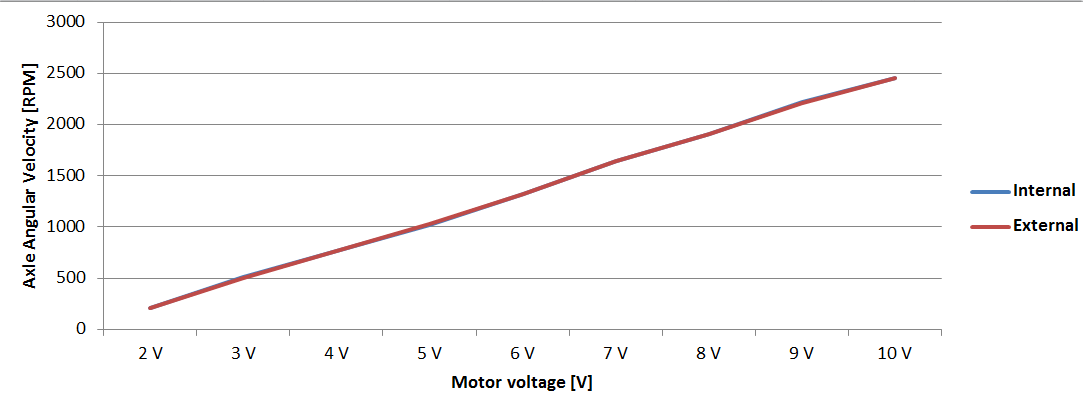
\includegraphics[width=\textwidth]{figures/appendix/Motor&GearTests/RPMTest}
	\caption{Plot of RPM found for both tachometers}\label{fig:RPMTest}
\end{figure}

\section*{Conclusion}
It its seen cf. figure \ref{fig:RPMTest} that the difference between the tachometers is so little, that the lines is on top of each other. The precision do not change with higher velocities and the internal tachometer is chosen, because it changes voltage faster because of the generator principle. The external optical tachometer needs some rotations to determine the RPM, and is not optimal when directions changes is needed.

